\documentclass[Bachelorarbeit.tex]{subfiles}
\begin{document}

\graphicspath{{./figures/appendixResults/}}	%specifying the folder for the figures

\chapter{Visual Results for Hub-Based, Scale-Free and Small-World Topologies}
  
\section{Hub-Based topologies} 
The Hub-Based Topologies fail to come even close to equilibrium due to reasons given in Chapter "Topologies and Hypothesis". This can be seen also very clearly in the visual results and thus no performance- and equilibrium-tables are listed as they would not make any sense.

\subsection{3-Hubs}
\begin{figure}[H]
	\centering
  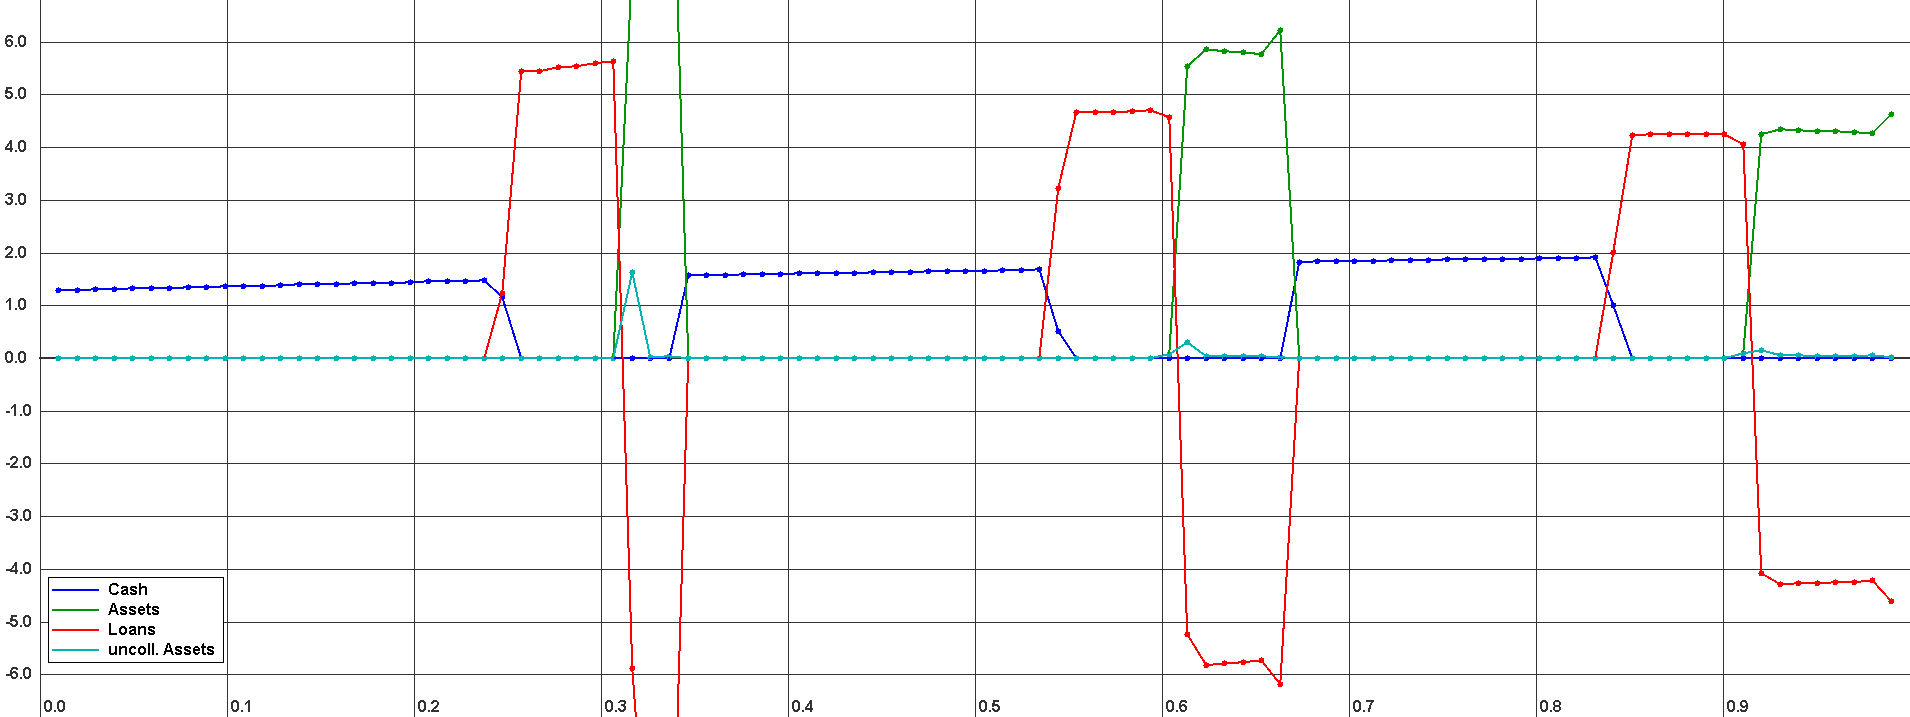
\includegraphics[width=1.0\textwidth, angle=0]{3HUBS_100_NOCOLLATERALMARKET_REPL.png}
	\caption{Wealth-Distribution of 3-Hubs topology}
	\label{fig1}
\end{figure}

\subsection{1-Median Hub}
\begin{figure}[H]
	\centering
  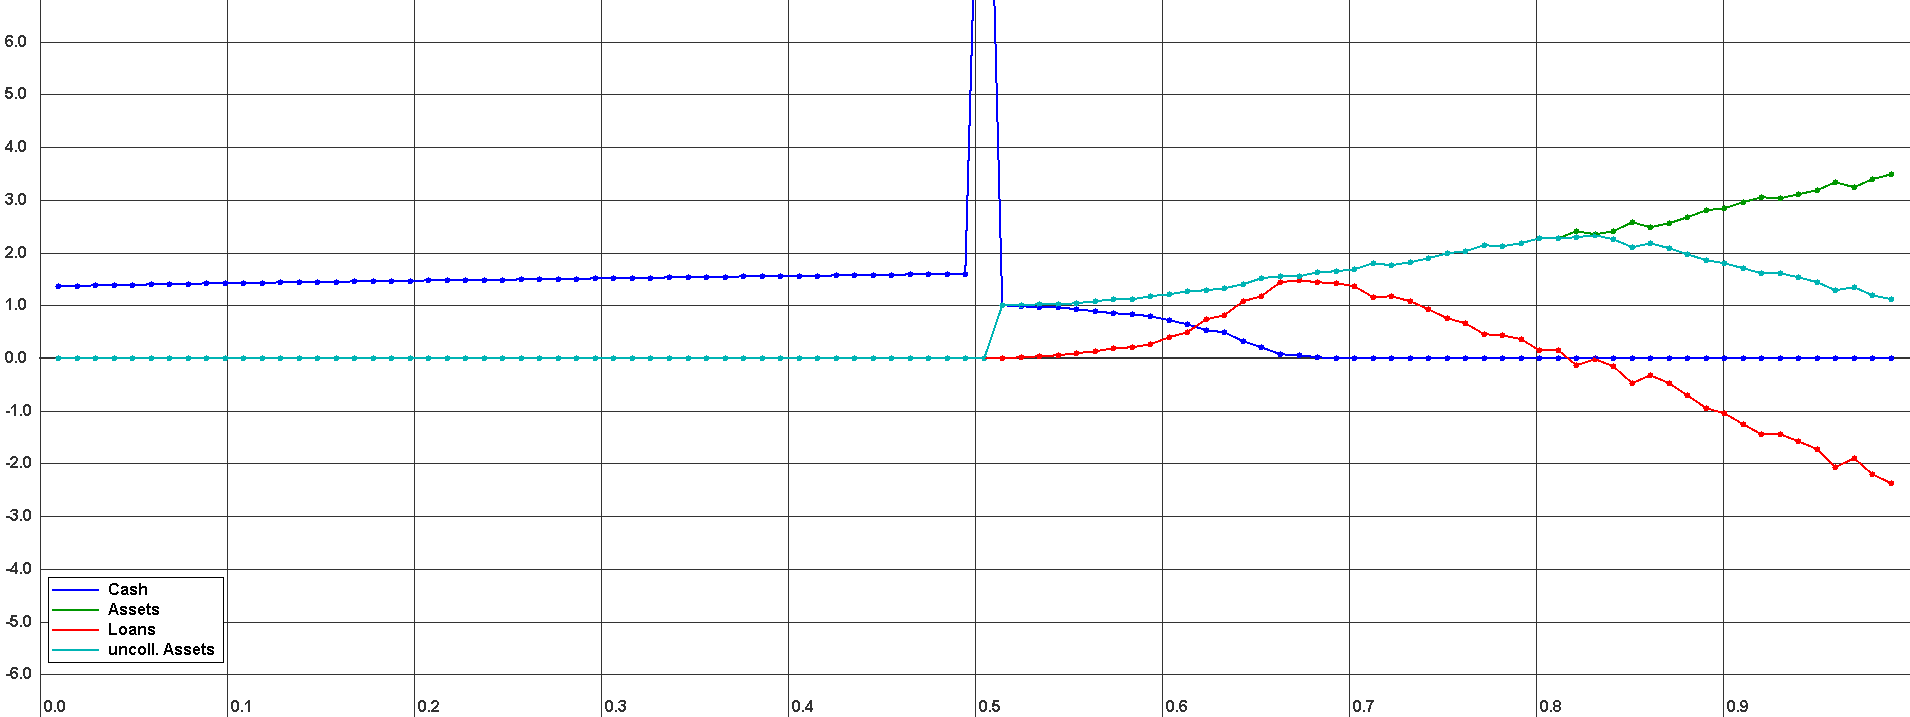
\includegraphics[width=1.0\textwidth, angle=0]{1MEDIANHUB_100_NOCOLLATERALMARKET_REPL.png}
	\caption{Wealth-Distribution of 1 Median-Hub topology}
	\label{fig1}
\end{figure}

\subsection{3-Median Hubs}
\begin{figure}[H]
	\centering
  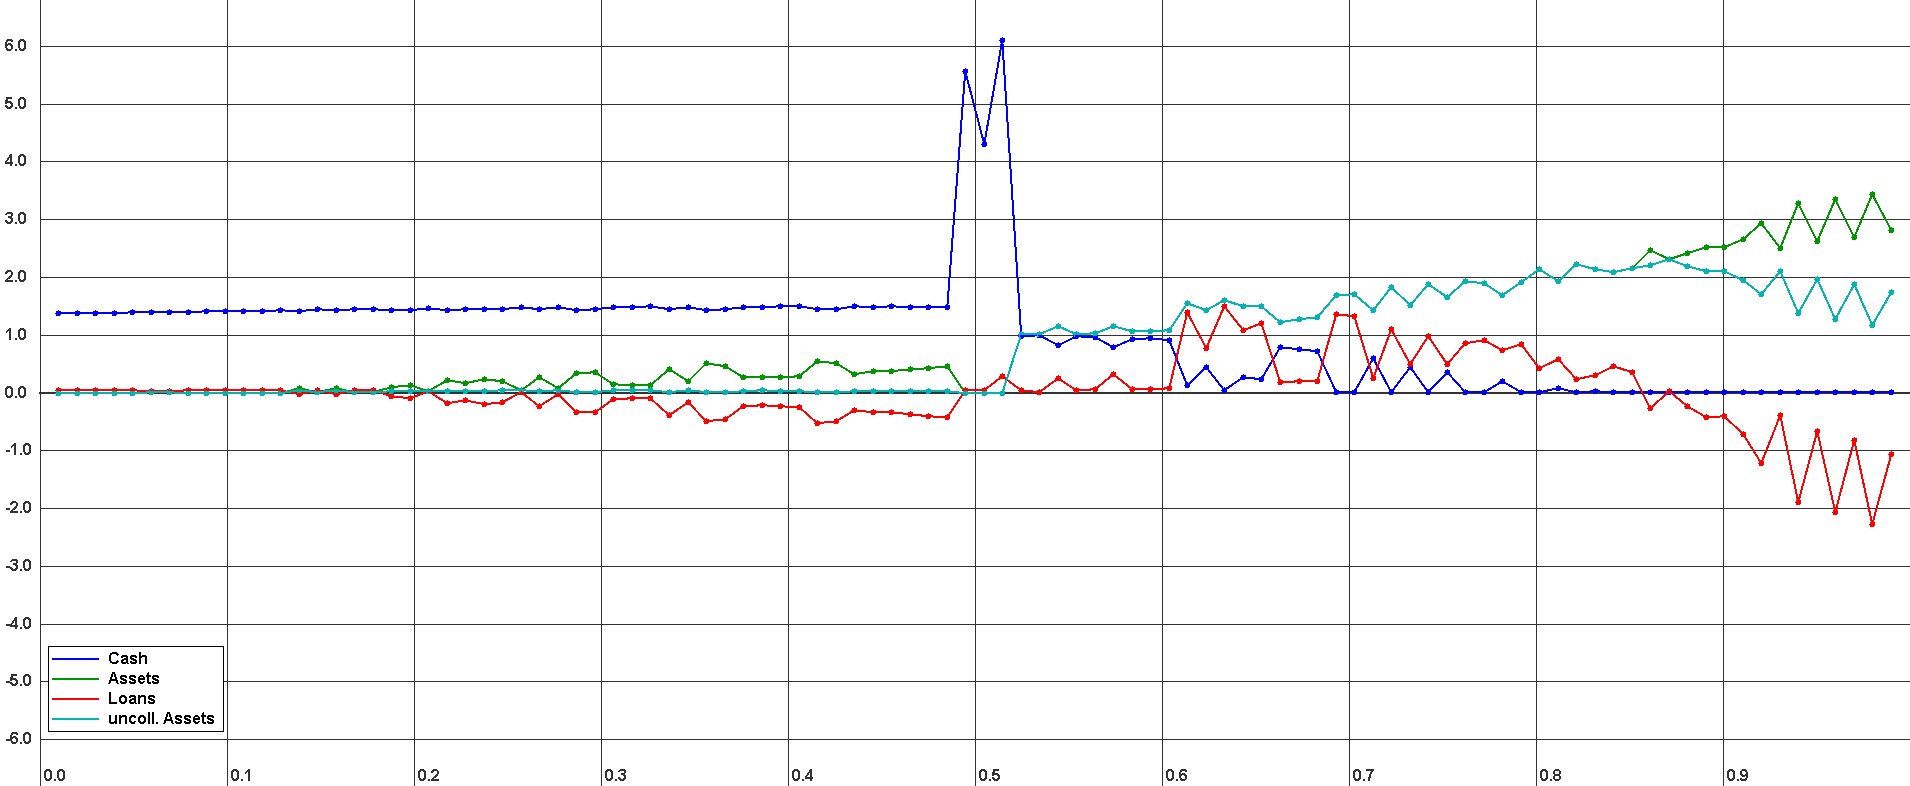
\includegraphics[width=1.0\textwidth, angle=0]{3MEDIANHUBS_100_NOCOLLATERALMARKET_REPL.png}
	\caption{Wealth-Distribution of 3 Median-Hubs topology}
	\label{fig1}
\end{figure}

\subsection{Maximum Hub}
\begin{figure}[H]
	\centering
  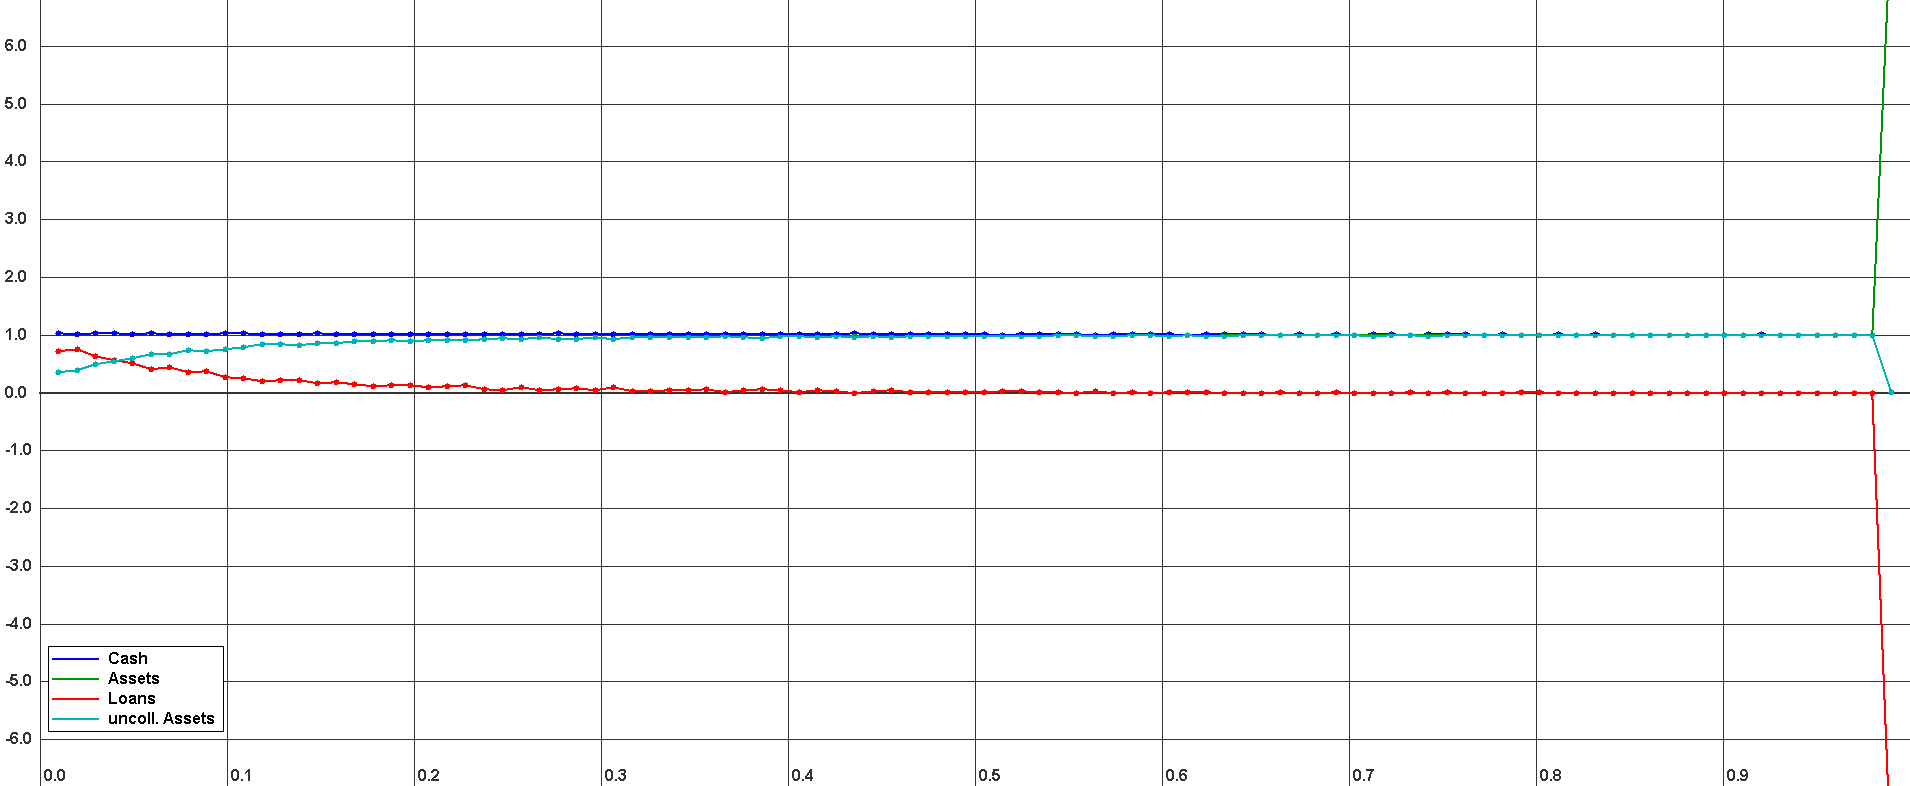
\includegraphics[width=1.0\textwidth, angle=0]{MAXIMUMHUB_100_NOCOLLATERALMARKET_REPL.png}
	\caption{Wealth-Distribution of Maximum-Hub topology}
	\label{fig1}
\end{figure}

\section{Scale-Free and Small-World topologies}
This topologies fail to come even close to equilibrium too due to reasons given in Chapter "Topologies and Hypothesis". This can be seen also very clearly in the visual results and thus no performance- and equilibrium-tables are listed as they would not make any sense.

\subsection{Erdos-Renyi}
\begin{figure}[H]
	\centering
  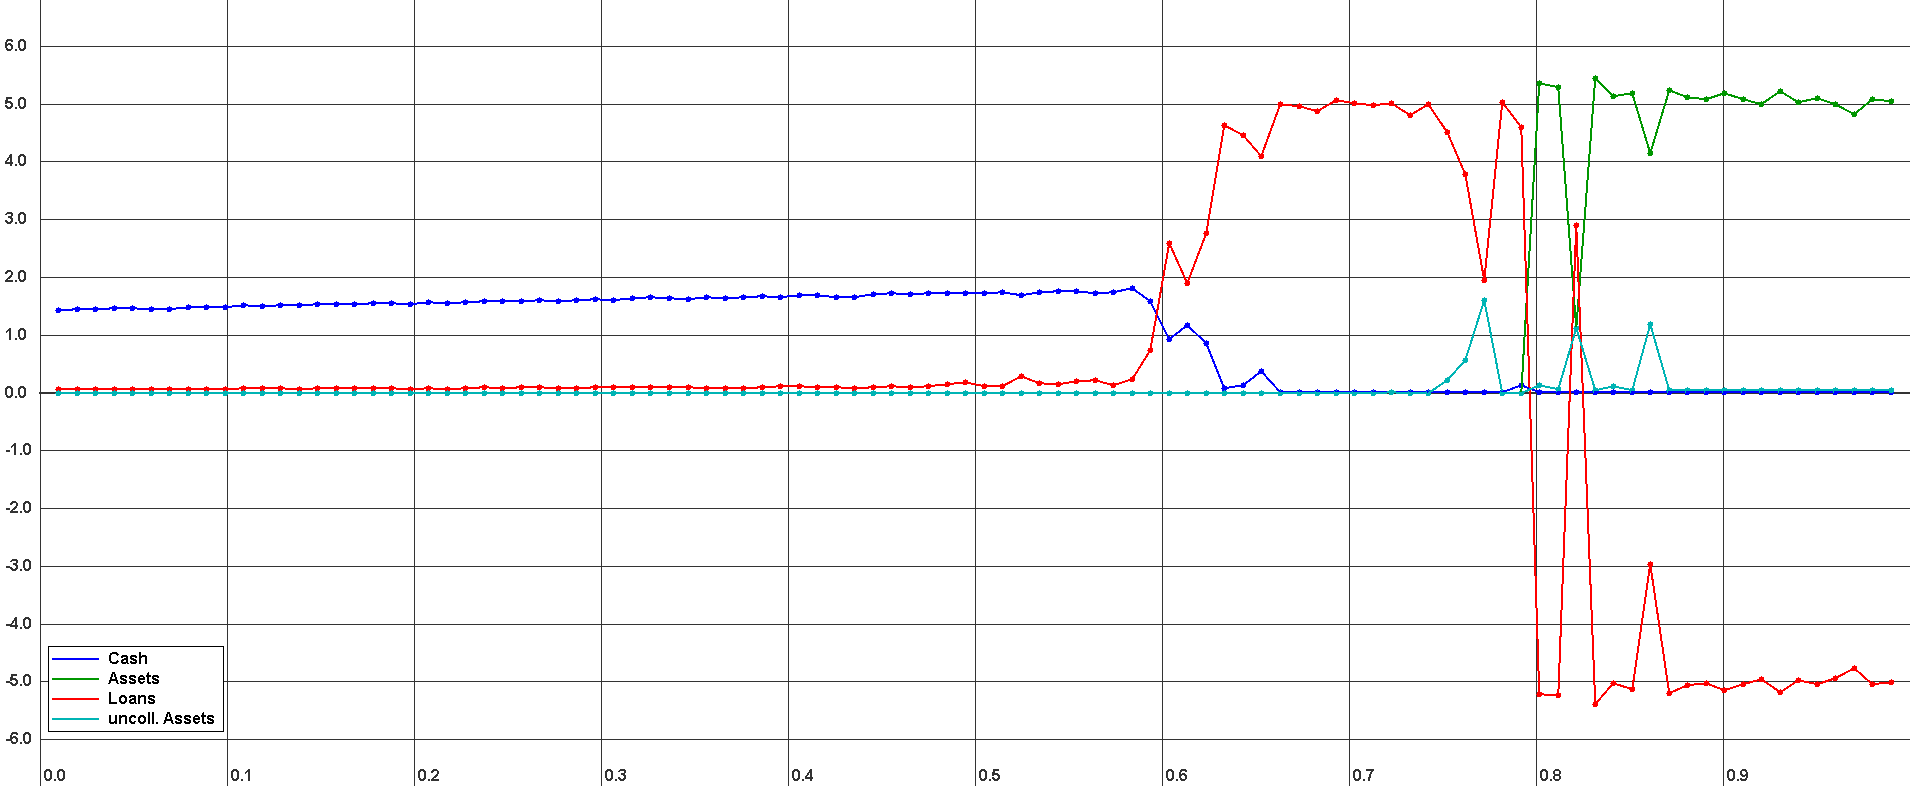
\includegraphics[width=1.0\textwidth, angle=0]{ERDOSRENYI_02_100_NOCOLLATERALMARKET_REPL.png}
	\caption{Wealth-Distribution of Erdos-Renyi 0.2 topology}
	\label{fig1}
\end{figure}

need to show network too because random ?

\begin{figure}[H]
	\centering
  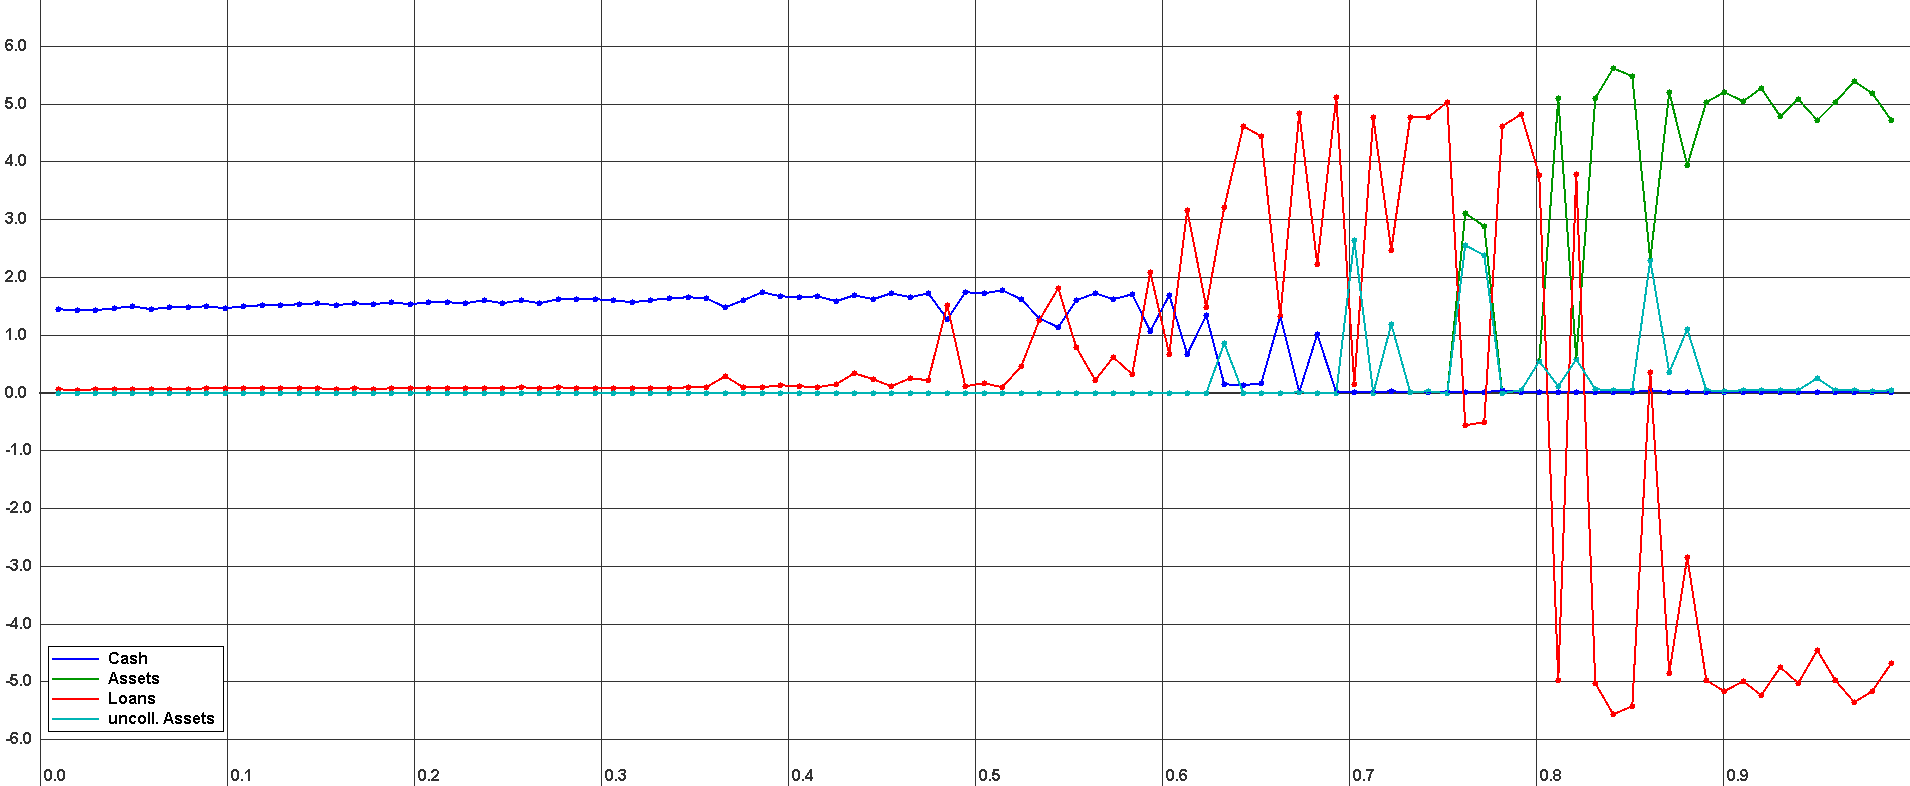
\includegraphics[width=1.0\textwidth, angle=0]{ERDOSRENYI_01_100_NOCOLLATERALMARKET_REPL.png}
	\caption{Wealth-Distribution of Erdos-Renyi 0.1 topology}
	\label{fig1}
\end{figure}

need to show network too because random ?

\begin{figure}[H]
	\centering
  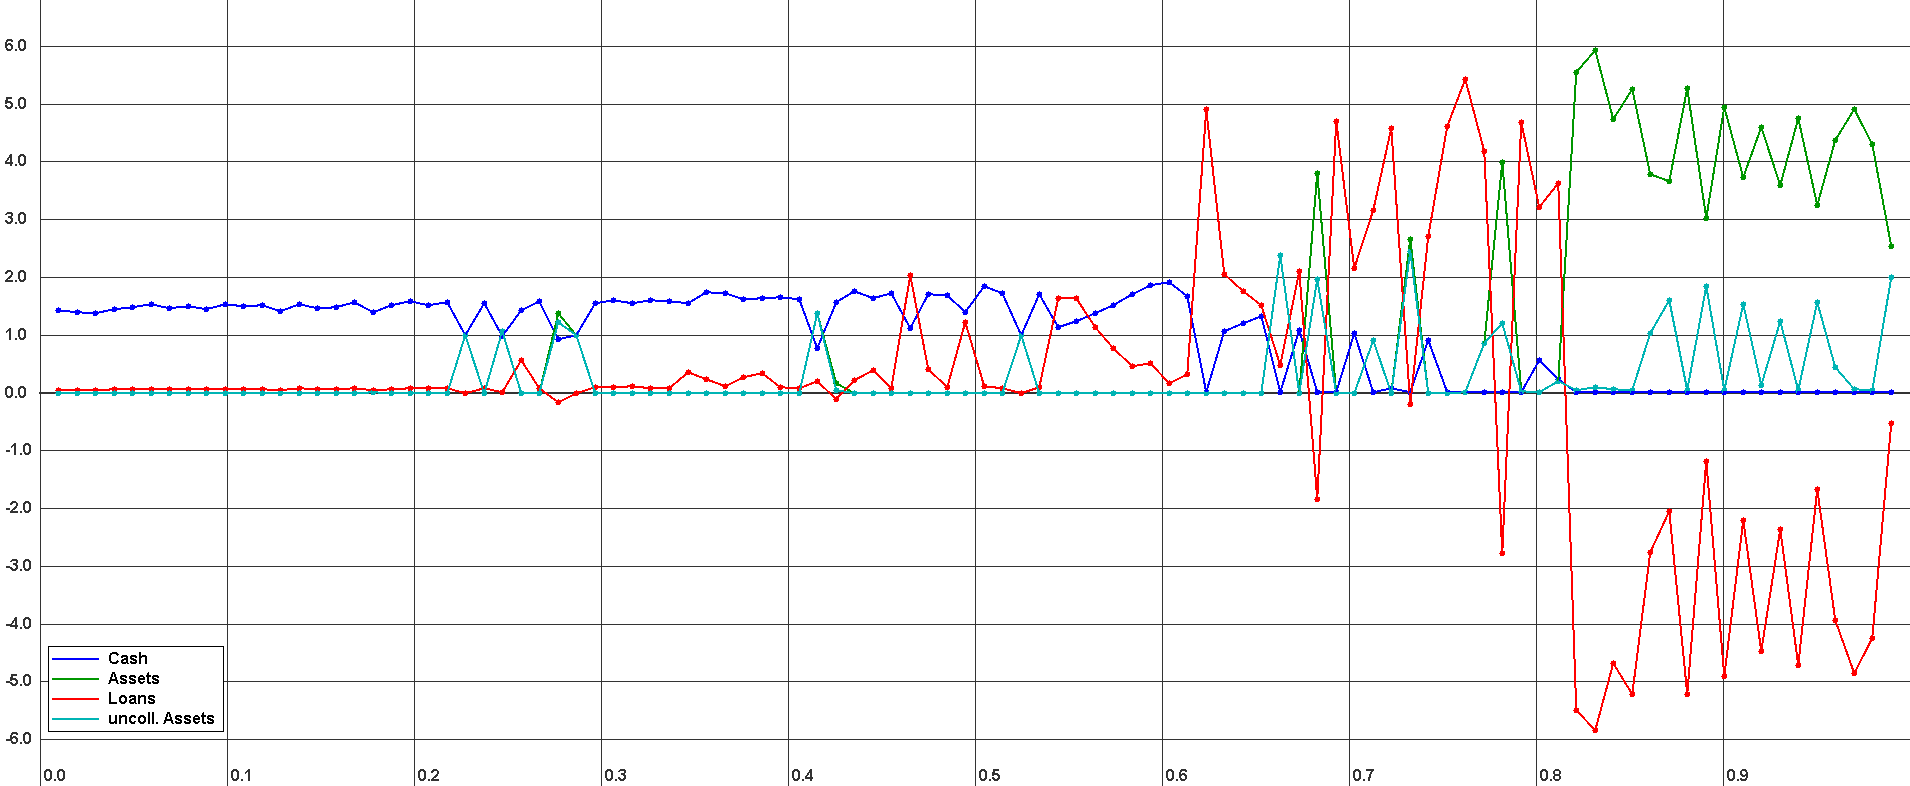
\includegraphics[width=1.0\textwidth, angle=0]{ERDOSRENYI_005_100_NOCOLLATERALMARKET_REPL.png}
	\caption{Wealth-Distribution of Erdos-Renyi 0.05 topology}
	\label{fig1}
\end{figure}

need to show network too because random ?

\subsection{Barbasi-Albert}
\begin{figure}[H]
	\centering
  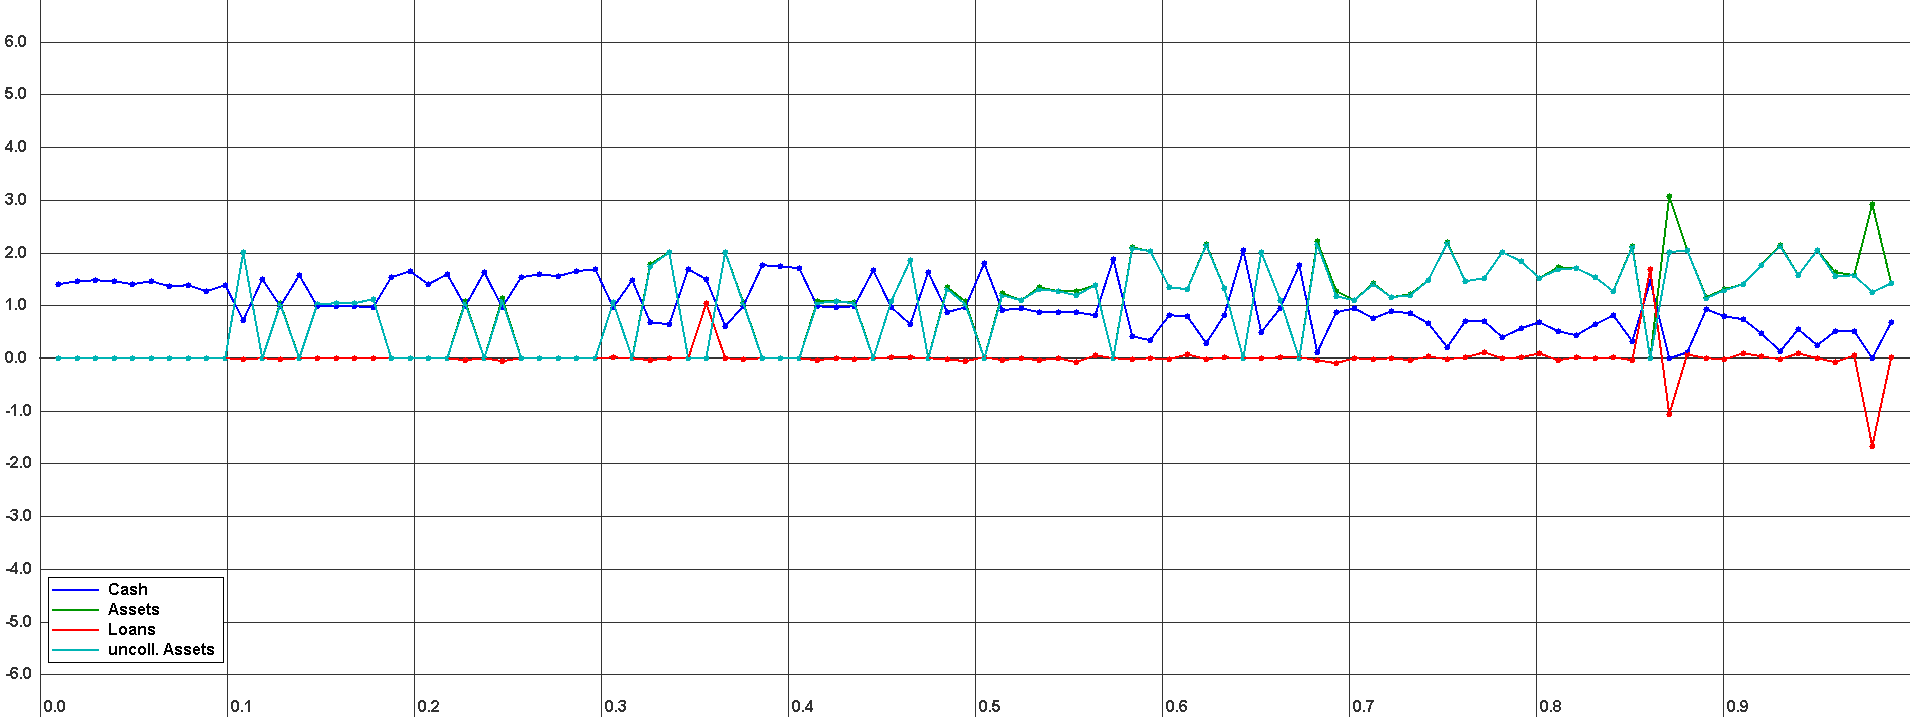
\includegraphics[width=1.0\textwidth, angle=0]{BARBASIALBERT_m03_m1_100_NOCOLLATERALMARKET_REPL.png}
	\caption{Wealth-Distribution of Barbasi-Albert m0=3, m=1 topology}
	\label{fig1}
\end{figure}

need to show network too because random ?

\begin{figure}[H]
	\centering
  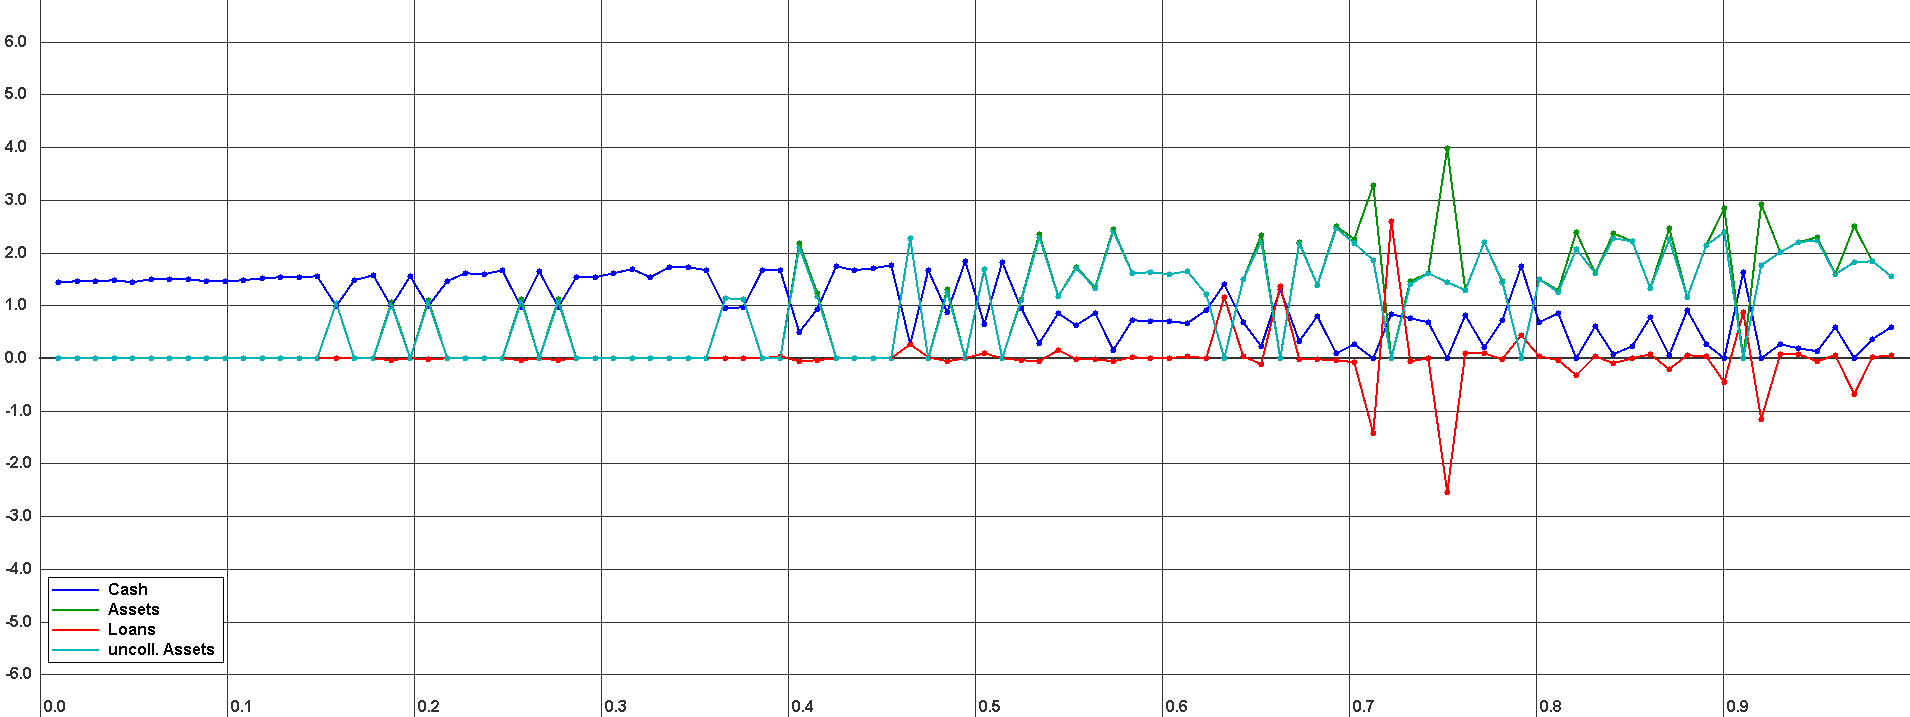
\includegraphics[width=1.0\textwidth, angle=0]{BARBASIALBERT_m09_m3_100_NOCOLLATERALMARKET_REPL.png}
	\caption{Wealth-Distribution of Barbasi-Albert m0=9, m=3 topology}
	\label{fig1}
\end{figure}

need to show network too because random ?

\subsection{Watts-Strogatz}
\begin{figure}[H]
	\centering
  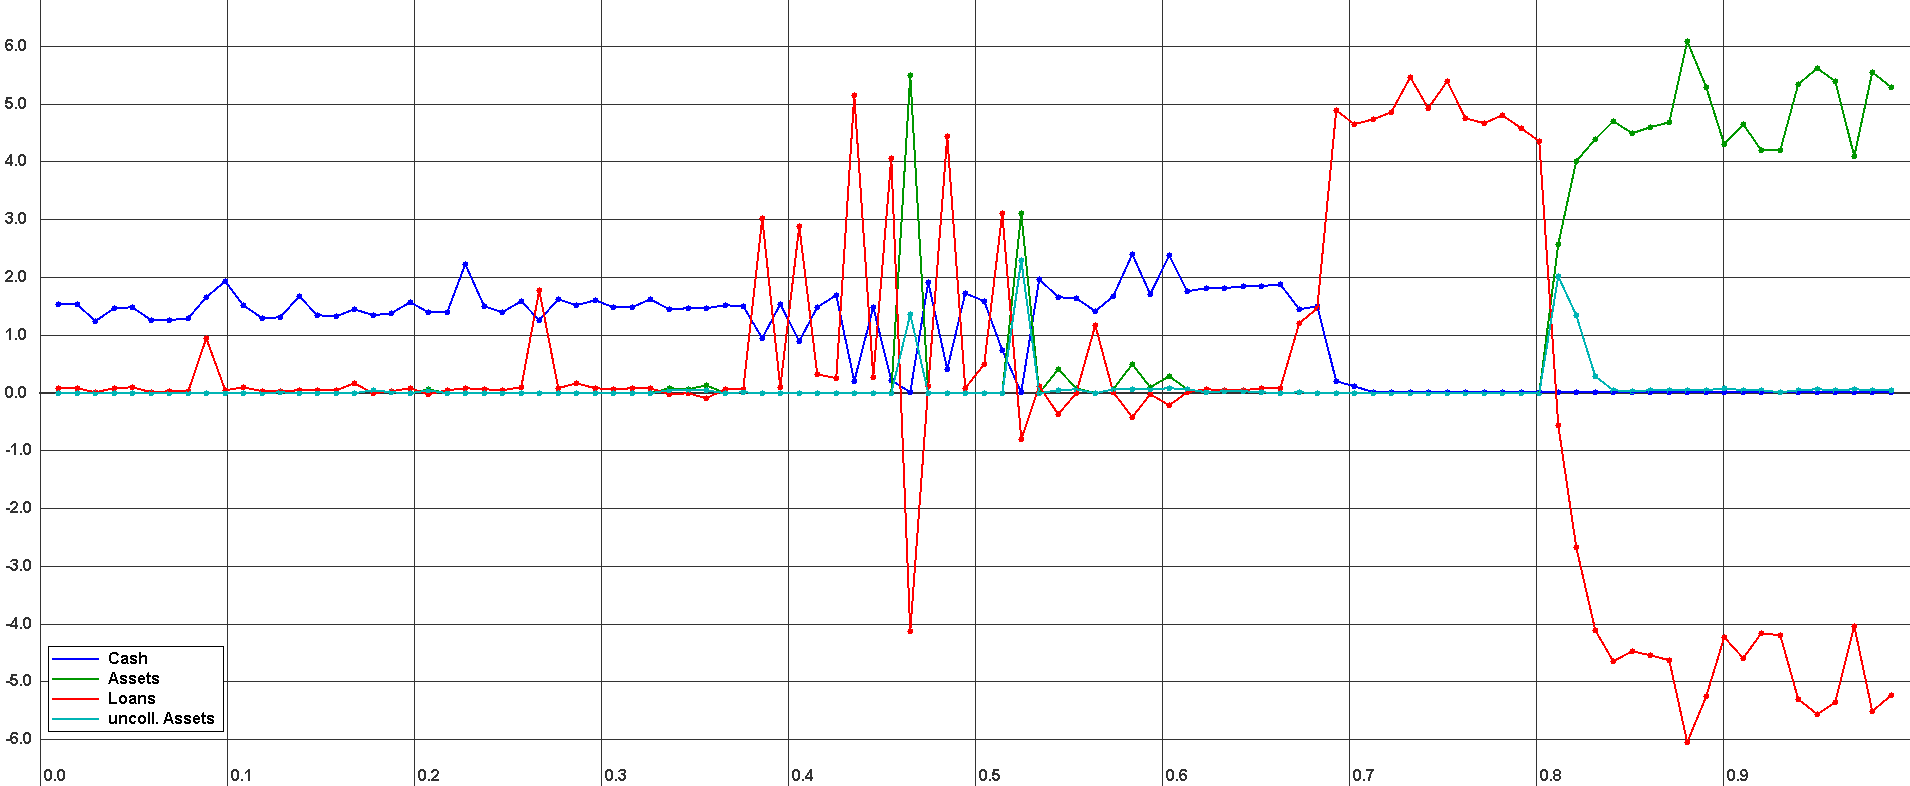
\includegraphics[width=1.0\textwidth, angle=0]{WATTSSTROGATZ_k2_b02_100_NOCOLLATERALMARKET_REPL.png}
	\caption{Wealth-Distribution of Watts-Strogatz k=2, b=0.2 topology}
	\label{fig1}
\end{figure}

need to show network too because random ?

\end{document}
